\documentclass[../TDE3.tex]{subfiles}%

\begin{document}
\section[s]"1"{Associations en parallèle}
% \subsection{Condensateurs}
\enonce{%
	On s'intéresse aux deux circuits ci-après, pour lesquels on ferme
	l'interrupteur $K$ à $t=0$. Les deux condensateurs sont initialement
	déchargés.
	\smallbreak
	\noindent
	\begin{minipage}[c]{0.40\linewidth}
		\begin{center}
			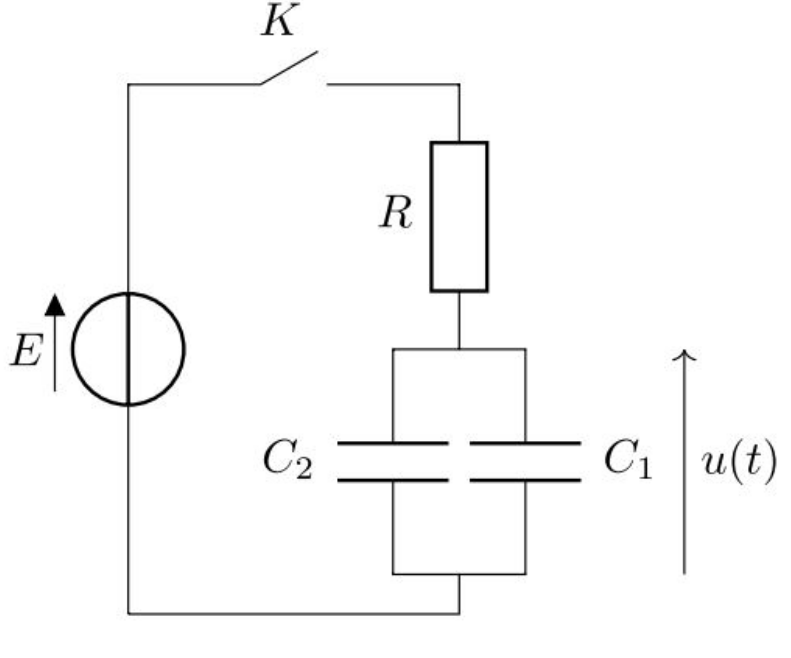
\includegraphics[width=.8\linewidth]{asso_parr-c}
			\captionof{figure}{1\ier{} montage.}
		\end{center}
	\end{minipage}
	\hfill
	\noindent
	\begin{minipage}[c]{0.40\linewidth}
		\begin{center}
			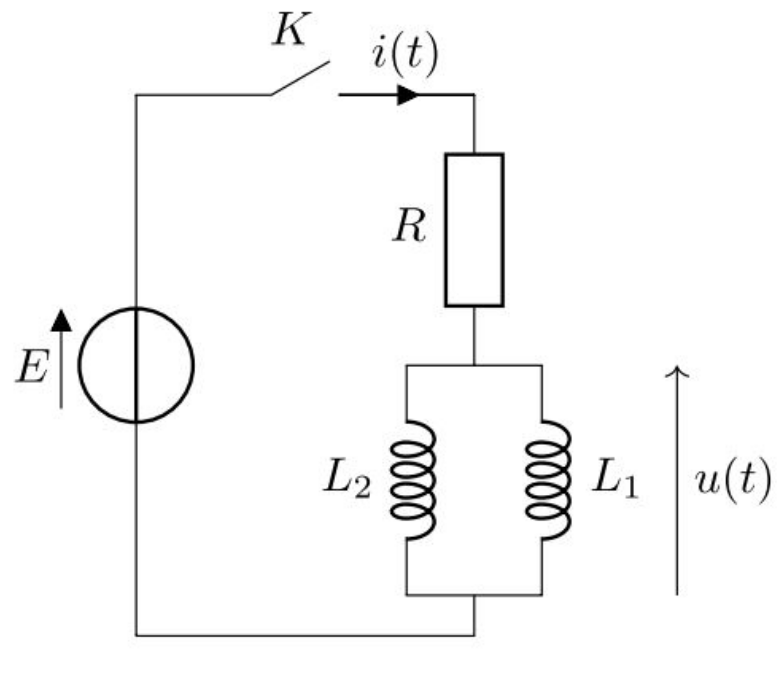
\includegraphics[width=.8\linewidth]{asso_parr-l}
			\captionof{figure}{2\up{d} montage.}
		\end{center}
	\end{minipage}
}
\QR{%
	Déterminer l'équation différentielle satisfaite par $u(t)$ pour le premier
	montage.
}{%
	Avec la loi des mailles et d'\textsc{Ohm}, puis la loi des nœuds~:
	% \beforetext{Loi des mailles et loi d'Ohm~:}
	% \beforetext{Loi des nœuds~:}
	\begin{DispWithArrows*}
		E & = Ri + u
		\tag{1}
		\label{eq:Cdeb}
		\\
		i & = i_1 + i_2
		\Arrow{RCT pour C}
		\\\Lra
		\dv{i}{t} & = C_1 \dv{u}{t} + C_2 \dv{u}{t}
		\\
		\text{Dans \eqref{eq:Cdeb}~:~}
		\Aboxed{%
			E & = R(C_1+C_2) \dv{u}{t} + u
		}%
	\end{DispWithArrows*}
}%
\QR{%
	À partir de cette équation, retrouver le composant équivalent aux deux
	condensateurs en parallèle.
}{%
	On constate qu'électriquement, l'association en parallèle donne un
	condensateur équivalent de capacité
	\[
		C_{\rm eq} = C_1 + C_2
	\]
}%

% \subsection{Bobines}
% \enonce{%
% 	\noindent
% 	\begin{minipage}{0.40\linewidth}
% 		\begin{center}
% 			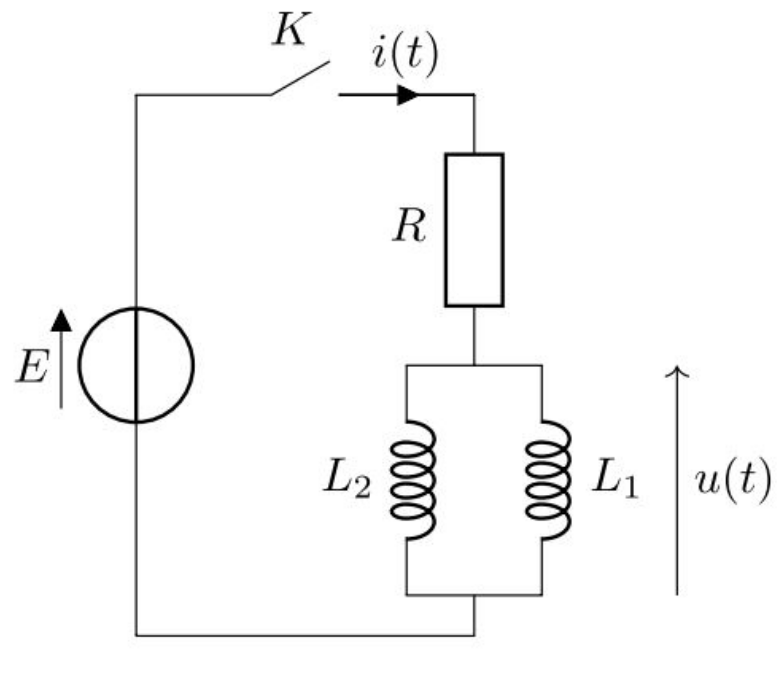
\includegraphics[width=.8\linewidth]{asso_parr-l}
% 		\end{center}
% 	\end{minipage}
% 	\hfill
% 	\noindent
% 	\begin{minipage}[c]{.55\linewidth}
% 		On considère le circuit ci-contre avec deux bobines différentes
% 		associées en parallèle. À $t=0$, on ferme l'interrupteur $K$.
% 	\end{minipage}
% }

\QR{%
	Déterminer l'équation différentielle satisfaite par $u(t)$ pour le second
	montage.
}{%
	\begin{DispWithArrows*}
		\text{Loi des mailles et loi d'Ohm~:~}
		E & = Ri + u
		\CArrow{$\dv{t}\/(\cdot)$}
		\\\Lra
		0 & = R \dv{i}{t} + \dv{u}{t}
		\tag{1}
		\label{eq:Ldeb}
		\\
		\text{Loi des nœuds~:~}
		i & = i_1 + i_2
		\CArrow{$\dv{t}\/(\cdot)$}
		\\\Ra
		\dv{i}{t} & = \dv{i_1}{t} + \dv{i_2}{t}
		\Arrow{RCT pour L}
		\\\Lra
		\dv{i}{t} & = \frac{u}{L_1} + \frac{u}{L_2}
		\\
		\text{Dans \eqref{eq:Ldeb}~:~}
		\Aboxed{%
			0 & = R\left(\frac{1}{L_1}+ \frac{1}{L_2}\right)u + \dv{u}{t}
		}%
	\end{DispWithArrows*}
}
\QR{%
	À partir de cette équation, retrouver un composant équivalent aux deux bobines
	en parallèle.
}{%
	On constate qu'électriquement, l'association en parallèle donne une bobine
	équivalente d'inductance
	\[
		\frac{1}{L_{\rm eq}} = \frac{1}{L_1} + \frac{1}{L_2}
	\]
}%

\end{document}
